\documentclass[19pt,a4paper]{article}
\usepackage{xeCJK}
\usepackage{amsmath}
\setmainfont{STSong}
\usepackage{geometry}
\geometry{left=2.5cm,right=2.5cm,top=2.5cm,bottom=2.5cm}
\setlength{\parindent}{4em}
\usepackage{graphicx}
\usepackage{float}
\title{算法作业9}
\author{孟妍廷2015202009}
\date{2017年11月29日}

\begin{document}
\maketitle
22.2-8\\
\indent 分析:首先一棵树应该是无向的,对于树T,其节点信息应该有如下两种情况:1.直接知道哪个结点是叶结点,哪个是根结点 2.只知道各个节点的邻接关系。对于两种情况设计算法如下:\\
\indent 1.直接知道根结点\\
假设根结点为s\\
$\indent solution1(T,s)\\
\indent \quad BFS(T,s)\\
\indent \quad D,d=-\infty\ \ //D是一个用于记录的空结点\\
\indent \quad for\ each\ v\in T.Adj[s]\\
\indent \quad\quad if\ v.d>D.d\\
\indent \quad\quad\quad D=v\\
\indent \quad return\ D$\\
\indent 时间复杂度为O(|V|+|E|)\\
\indent 2.只知道邻接关系\\
借助1中的算法solution1\\
$\indent solution2(T)\\
\indent \quad // 任意选取树中的一个结点u\\
\indent \quad s=solution1(T,u)//先找到任意一个节点u的最短路径距离最长的结点s,s一定为直径的一端\\
\indent \quad D=solution1(T,s)//以端点开始执行BFS找最短路径最长结点即为目标\\
\indent \quad return\ D$\\
\indent 时间复杂度为O(|V|+|E|)\\
\indent 22.3-11\\
\indent 分析:首先唯一结点的意思是指该节点没有树边与其他结点连接,与选择节点的顺序造成的开始时间和完成时间有关。考虑具有如下性质的结点u
\begin{figure}[H]
\centering
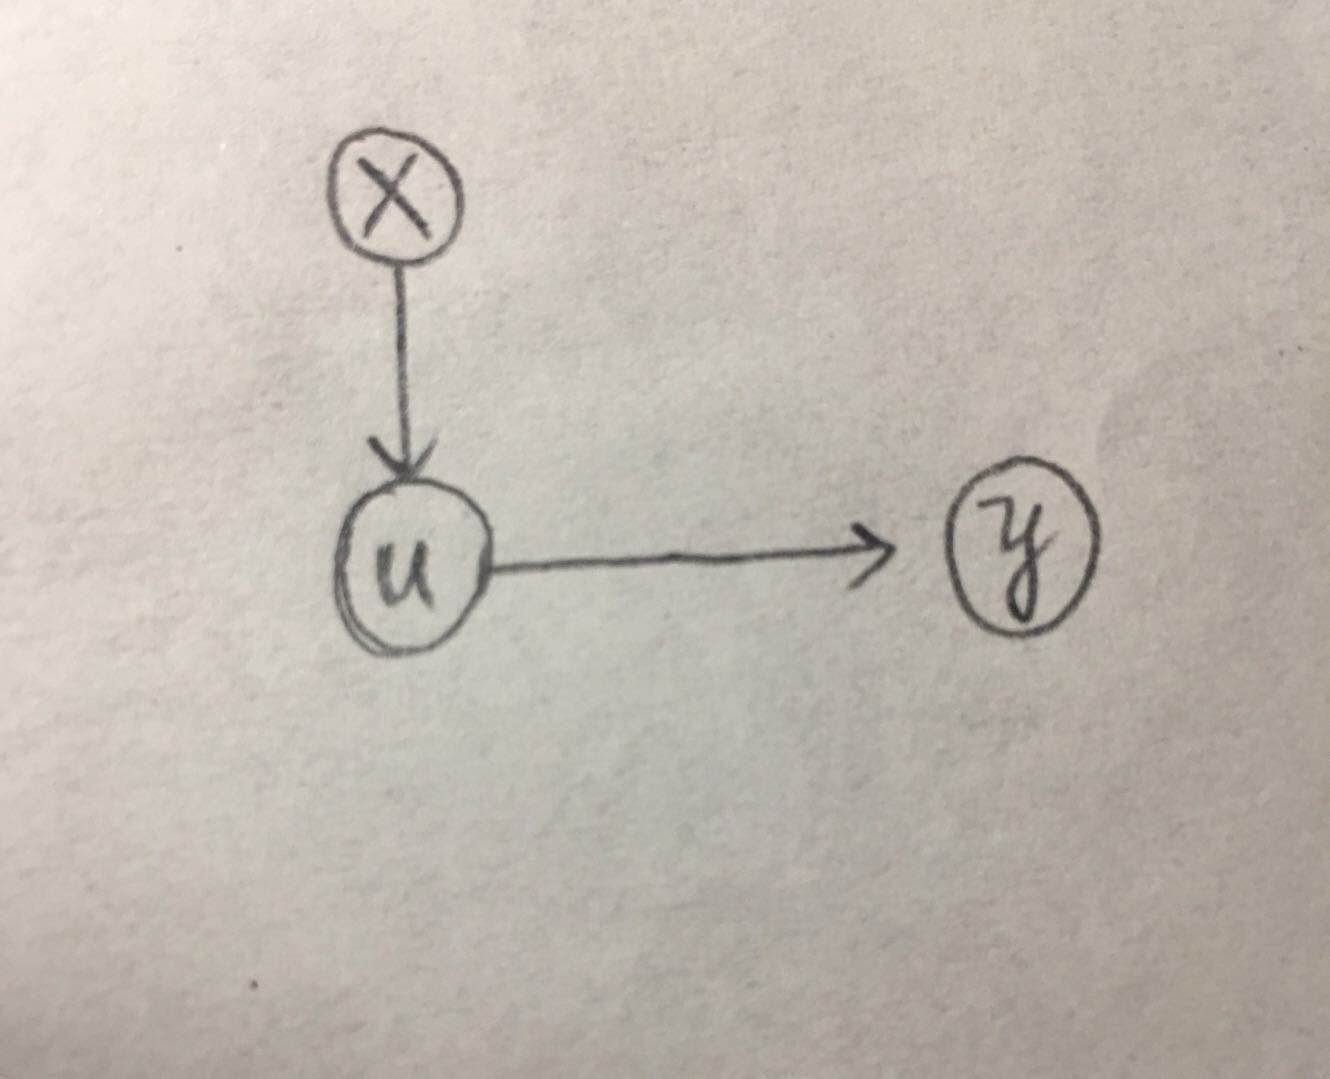
\includegraphics[scale=0.2]{91.jpeg}
\end{figure}
\indent 按照一定顺序选取结点进行深度优先算法,可得各结点的开始时间和结束时间如下:
\begin{figure}[H]
\centering
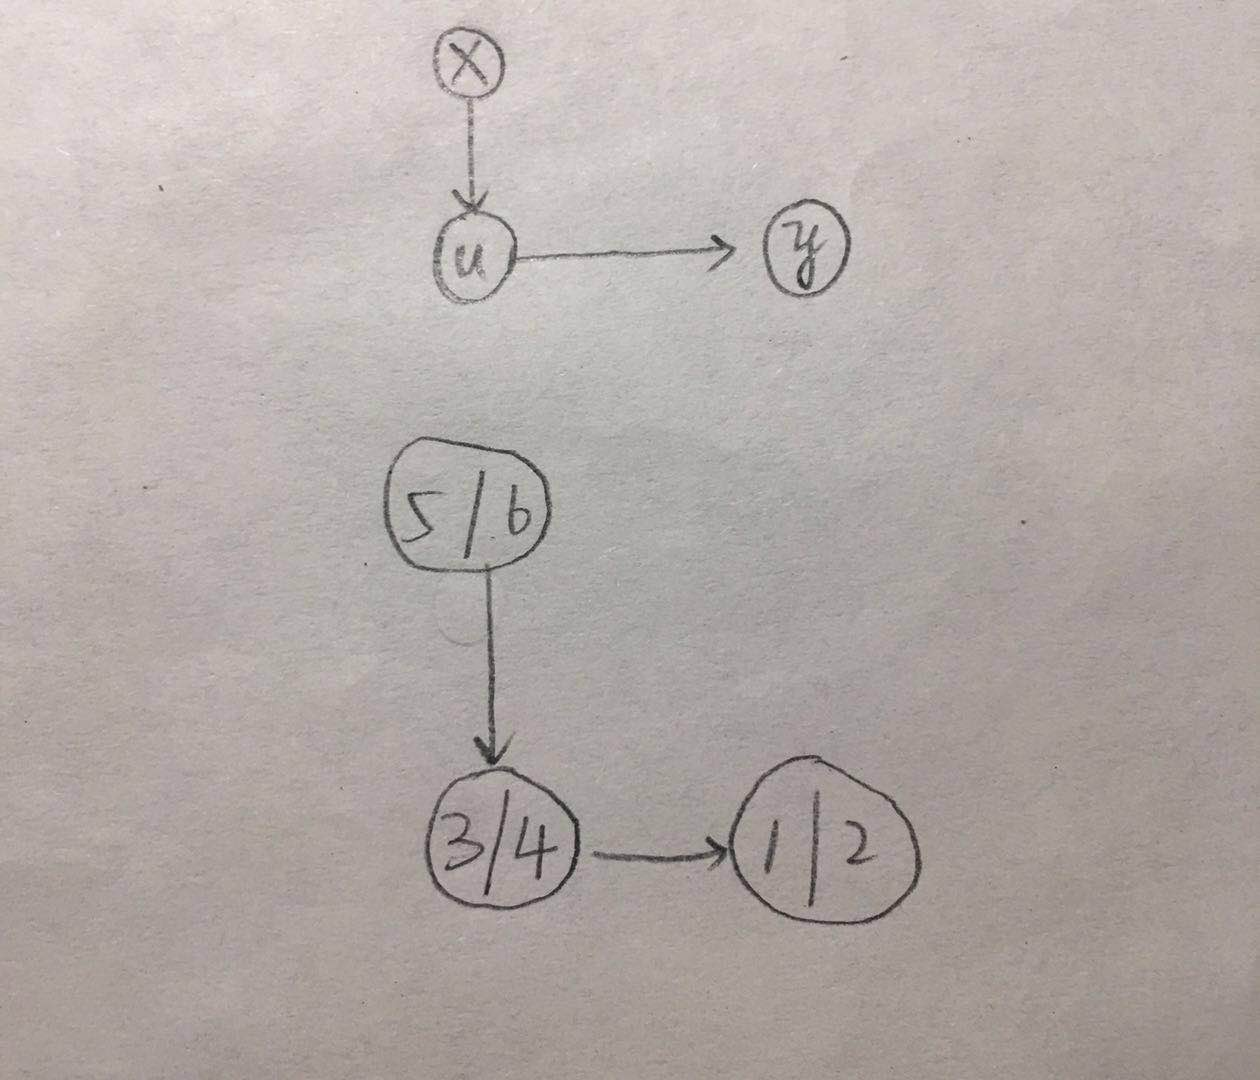
\includegraphics[scale=0.2]{92.jpeg}
\end{figure}
\indent 也就是说,对于既有出边也有入边的结点u,若进行深度优先算法使其出边指向的结点在它被选择之前就被选择,而指向它的结点
在它之后被选择就会使其成为唯一节点\\
\indent 因此具有这样的结构的既有出边也有入边的结点u能成为深度优先树中的唯一节点。\\
\indent 22.5-3\\
\indent 解:不一定能计算出结果。以书上的例子作为反例
\begin{figure}[H]
\centering
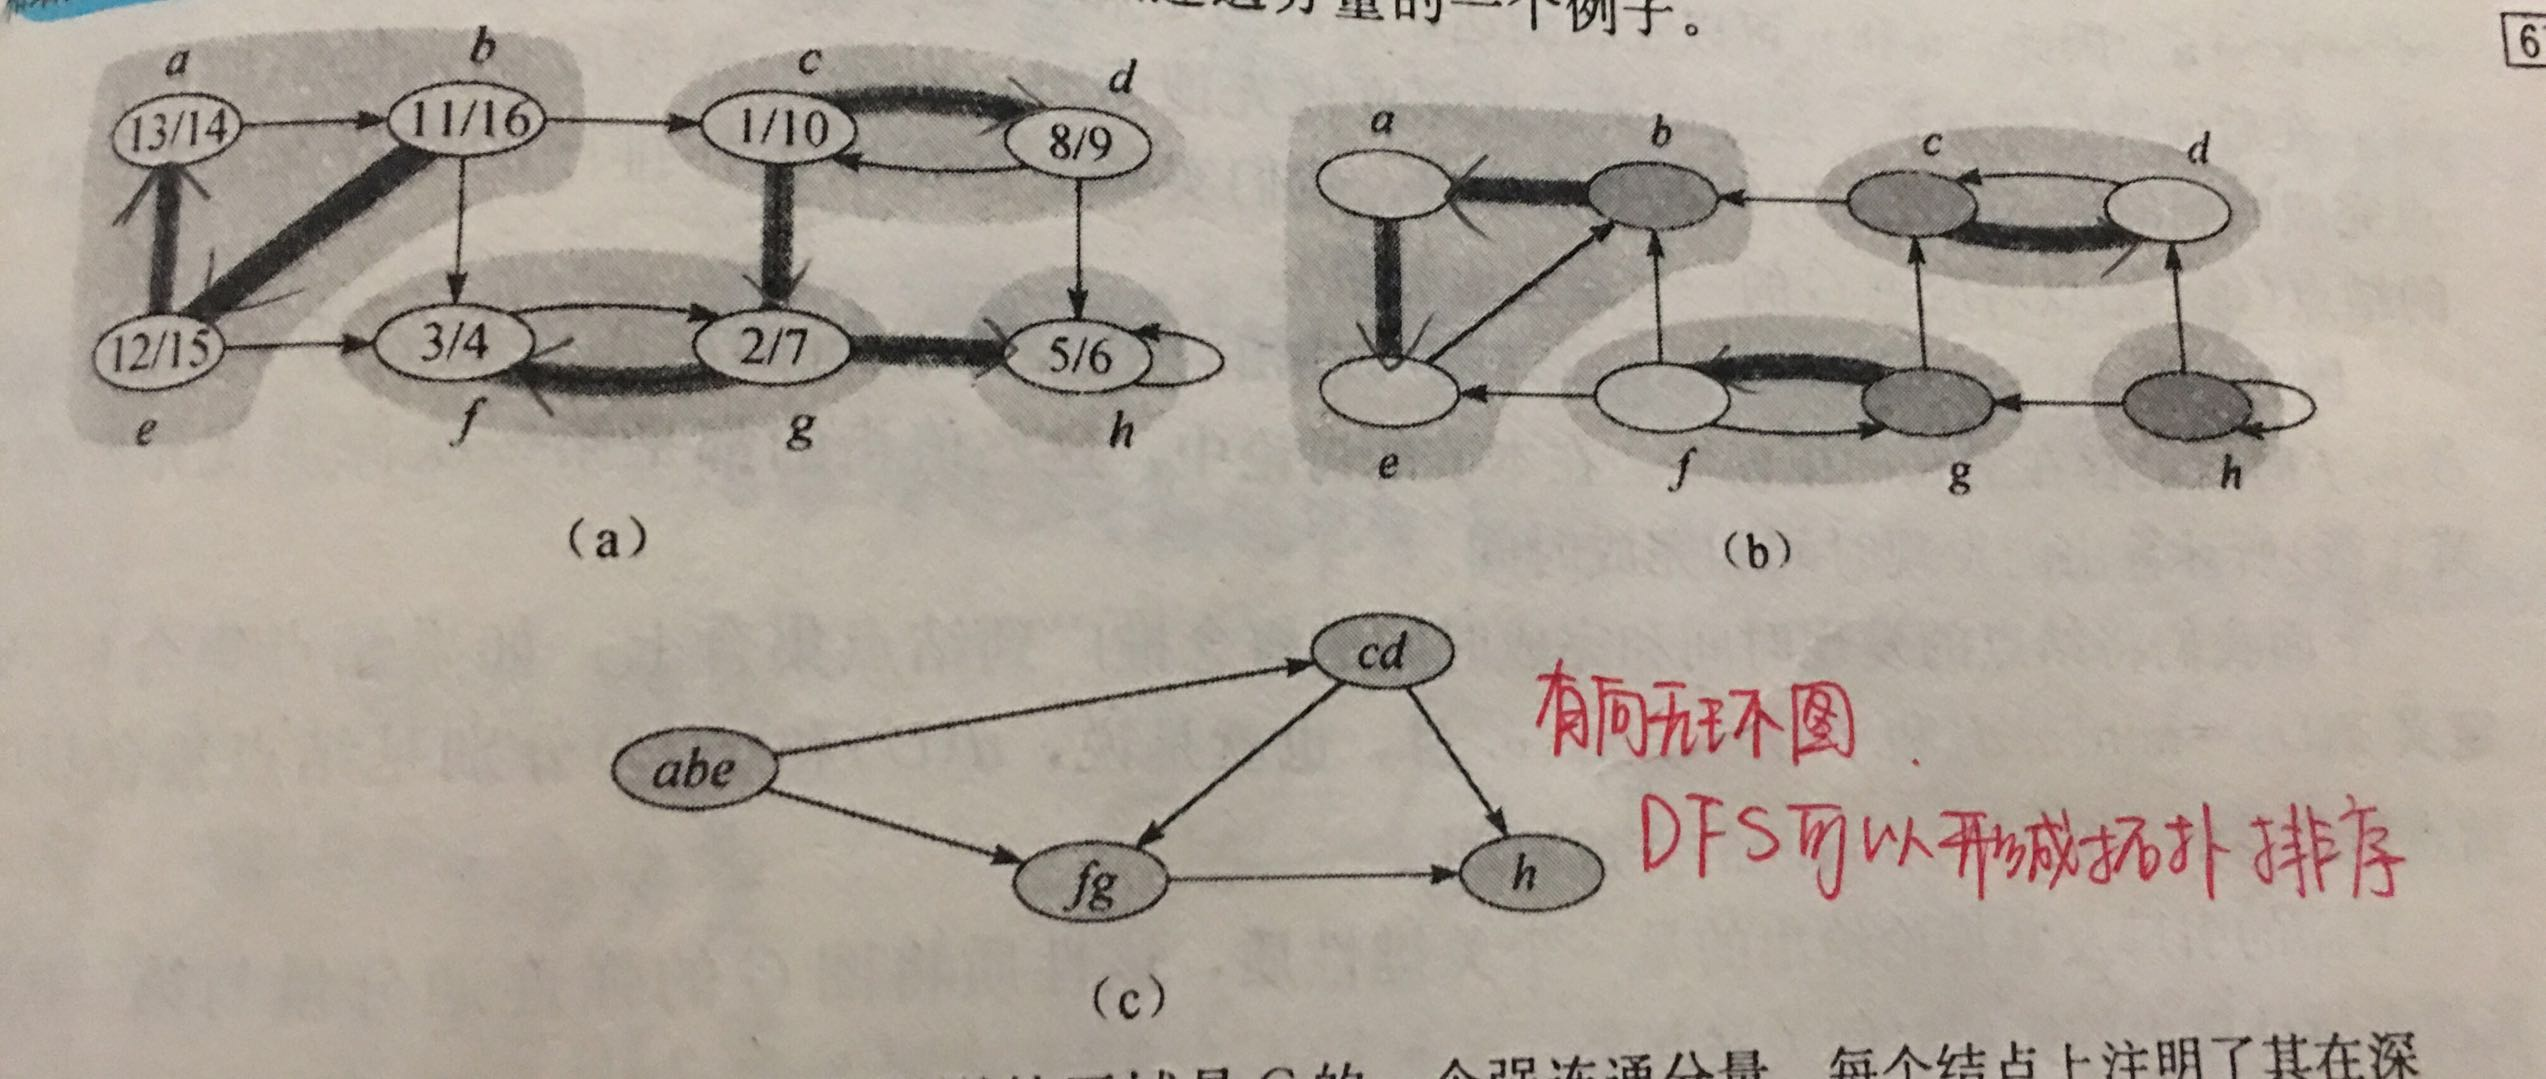
\includegraphics[scale=0.2]{93.jpeg}
\end{figure}
\indent 若不转置,从结束时间最短的结点开始正序遍历,则第一个选择的结点为f,f指向g,此时g既可以指向f也可以指向h,产生的冲突,并不能保证一定能形成强连通图。


\end{document}